\chapter{Phase Transitions}
    By Gibbs' definition, \textbf{phase} is a state of matter, which is uniform throughout, both in chemical and physical sense. By outside influence, phase of the system can change in a \textbf{phase transition}. Phase transition manifests itself as an abrupt change in one or more properties of the system. For example, in a material transitioning to a superconductor, the electrical resistivity goes from a finite number to zero. During the phase transition, two phases can coexist separated by a boundary. This is called the \textbf{phase separation}. 
    \section{Thermodynamic Potential}
        Consider a system of $N_A$ identical particles, placed in a heat bath with temperature $T_R$ and pressure $P_R$. The equilibrium is identified as the state which minimises the thermodynamical potential. For constant pressure and a fixed number of particles,\begin{equation}
            G = U_A + P_RV_A-T_RS_A.
        \end{equation}
        Minimising this function with respect to the internal energy and volume,
        \begin{equation}
            \frac{\del G}{\del U_A} = 1 - T_R \frac{\del S_A}{\del U_A} = 1-\frac{T_R}{T_A}.
        \end{equation}
        This is zero when $T_R=T_A$, i.e. when the temperatures of the system and the reservoir are equal. Differentiating with respect to volume,
        \begin{equation}
            \frac{\del G}{\del V_A} = P_R -T_R \frac{\del S_A}{\del V_A}=P_R-\frac{T_R}{T_A}P_A,
        \end{equation}
        which is zero when $T_A=T_R$ and $P_A=P_R$. Then, we can define the thermodynamic potential as a function of state that gets minimised under a certain set of constraints. We now define a \textbf{generalised thermodynamic potential}, $\Phi(\phi)$ where $\phi$ is a variable quantity. For example, if the thermodynamic potential is the grand potential, then $\phi = N$. To simplify, we can set that $\Phi$ depends only on the average value of $\phi$ and not the fluctuations in its value. \\
        \\
        $\Phi(\phi)$ can have one or multiple local minima. An example is water and water vapour. These are the two phases of the same material, $H_2O$, which correspond to two different minima of the potential. At low temperatures, the minima (well) corresponding to the water is more favourable. However, as temperature increases, the vapour well becomes more favourable.\\
        \\
        Consider the thermodynamic potential $\Phi(x_1,x_2,...)$ which depends on all constrained parameters, $x_i$. If any of the derivatives $\del_i\Phi$ are discontinous at the transition, then we have a \textbf{first-order transition}. If however, all derivatives are continous, we get a \textbf{second-order phase transition}. Second-order transitions are also called continous transitions. As an example, consider the Gibbs free energy. We have $x_1 =T$ and $x_2=P$. 
        \begin{equation}
            S = - \lrp{\frac{\del G}{\del T}}_P \hspace{0.5cm} V = \lrp{\frac{\del G}{\del P}}_T
        \end{equation}
        If we consider the two entropies corresponding to the two wells,
        \begin{equation}
            S_1=-lrp{\frac{\del \Phi}{\del T}}_{P,1} \hspace*{0.5cm} S_2=-\lrp{\frac{\del \Phi}{\del T}}_{P,2}.
        \end{equation}
        Here, the entropies may be different. The difference between the entropies gives the \textbf{latent heat}. For $T_p$ the transition temperature, latent heat is given by
        \begin{equation}
            L_{1,2} := T_p(S_1-S_2).
        \end{equation}
        In general, well defined boundaries exist between regions where different phases are stable. These boundaries can be seen in \textbf{phase diagrams.}
        \begin{figure}[h!]
           \centering
           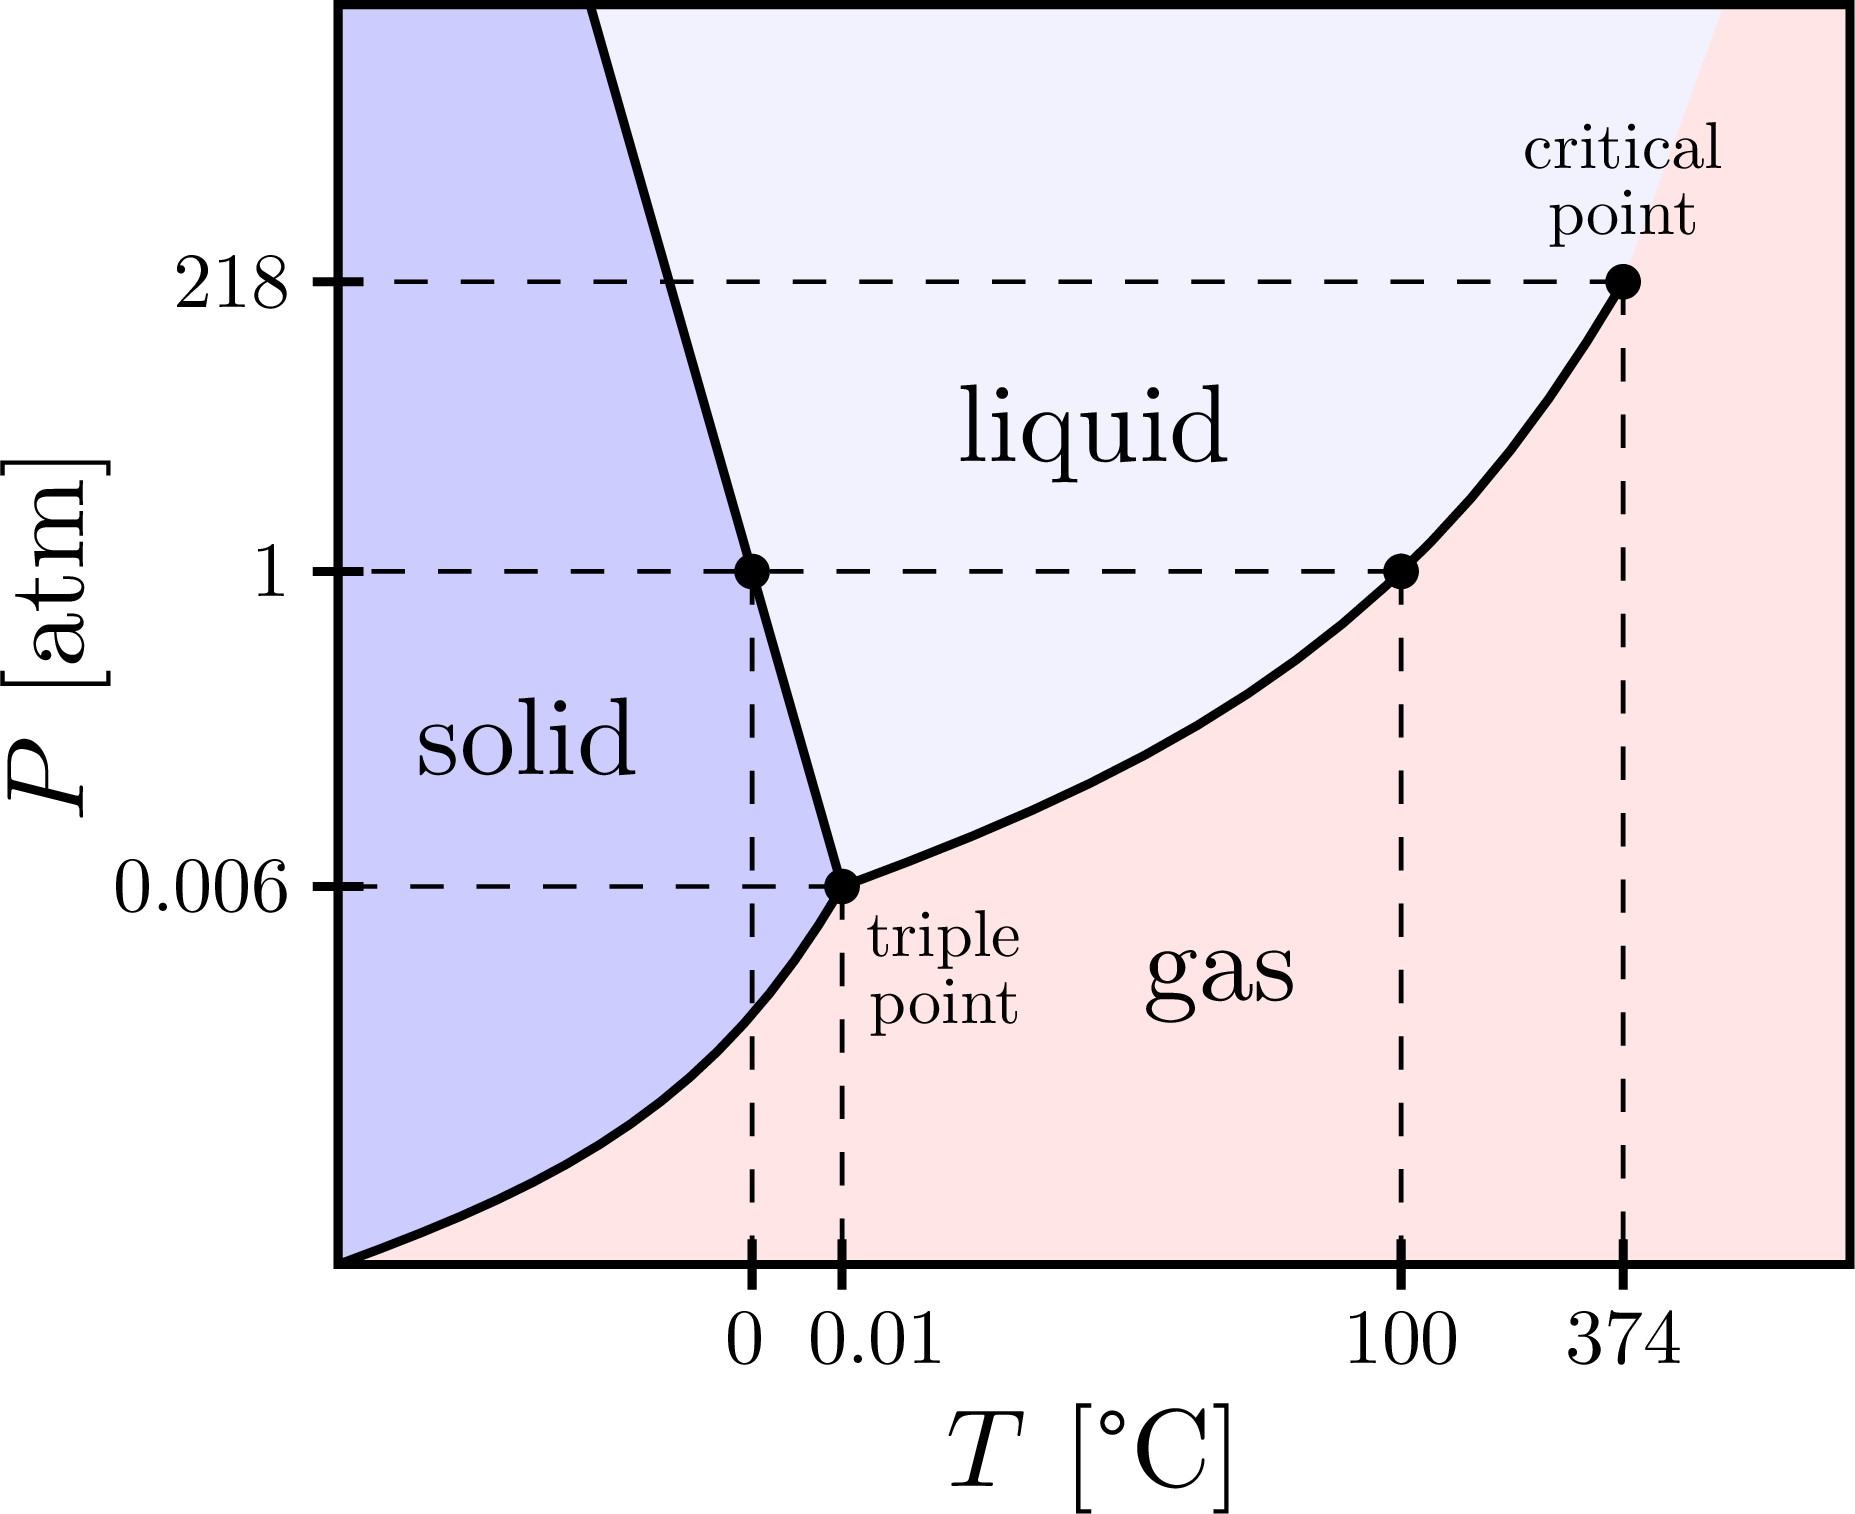
\includegraphics[width=0.5\linewidth]{phasediagram.png}
           \caption{The phase diagram of the water.}
           \label{fig:phasediagram}
        \end{figure}

        On the boundary lines, the phases are equally stable. The point where all three major phases (solid, liquid, and gas) are stable is called the \textbf{triple point}. If a system crosses a boundary, then a first-order transition occurs. \\
        \\
        First-order transitions also display \textbf{metastability}. Consider a potential with two wells. Initially, well 2 is favoured. As the temperature increases, the minimum of well 2 becomes higher than that of the well 1. At that point, well 2 becomes metastable. By crossing a free-energy barrier via thermal activation, the system goes from the well 2 phase to well 1 phase. If the barrier is considerably larger than the $k_BT$ of the system, this activation can take time. However, as the system is cooled, the barrier shrinks to zero. Then, the system rapidly moves to well 1. \\
        If the barrier is sufficiently large, the metastable state persists indefinetly. Then, the metastable state seems to be a thermodynamically stable.  \\
        \\
        A liquid can be cooled below its solidification temperature and can remain a liquid until a solid is nucleated and spreads. At this state, the liquid is said to be \textbf{supercooled}. A supercooled liquid is a metastable state and this stability can last until a nucleus is formed either by further cooling or by artificially planted. \\
        The lowest temperature that a supercooled liquid can reach before the solid phase is formed is lower than the actual solidifcation temperature. If we were to take the system around a cycle in which the solid is first heated and then cooled, we would obtain two different estimates of the transition temperature. For the same temperature, we could either have a solid or a supercooled liquid depending on the point in the cycle. This behaviour is known as \textbf{hysteresis}.

        \section{Clapeyron Equation}
            If two coexisting phases are in equilibrium, i.e. $\mu_1=\mu_2$ and $G_1=G_2$ and we consider two nearby points on the phase boundary line, $(P,T)$ and $(P+dP,T+dT)$, then
            \begin{align}
                G_1(T,P) =& G_2(T,P) \\
                G_1(T+dT,P+dP) =& G_2(T+dT,P+dP)
            \end{align}
            If we expand (11.2.2) in Taylor series,
            \begin{equation}
                G_1(T,P) + \frac{\del G_1}{\del T} dT + \frac{\del G_1}{\del P}dP = G_2(T,P)+\frac{\del G_2}{\del T}dT + \frac{\del G_2}{\del P}dP.
            \end{equation}
            Rearranging gives
            \begin{equation}
                \lrp{\frac{\del G_1}{\del P}-\frac{\del G_2}{\del P}}dP = -\lrp{\frac{\del G_1}{\del T}-\frac{\del G_2}{\del T}}dT.
            \end{equation}
            From $dG = -SdT + VdP$, (11.2.4) becomes
            \begin{equation}
                \frac{dP}{dT}=-\frac{\frac{\del G_1}{\del T}-\frac{\del G_2}{\del T}}{\frac{\del G_1}{\del P}-\frac{\del G_2}{\del P}} = \frac{S_1-S_2}{V_1-V_2} = \frac{L_{12}}{T_p\Delta V}.
            \end{equation}
            This is the \textbf{Clapeyron equation}.
            \begin{equation}
                \frac{dP}{dT} = \frac{L_{12}}{T_p\Delta V}
            \end{equation}

        \section{Phase Separation}
            Consider two experiments. In one, there is a movable piston while in the other, the piston is fixed. In the first experiment, lowering the temperature will cause the volume and thus the density to change whereas in the second one, the density will remain fixed as the volume does not change. If the system cannot lower the density, then it can minimise the potential $\Phi$ via phase separation. Let $\phi$ be the fixed variable and imagine a two-well problem. \\
            Since it is fixed, the average value of $\phi$ must be constant. Let $x$ be the fraction of the system which sits in well 1. Then the fraction of the system which sits in well 2 is $1-x$. Since $\bar{\phi}$ is constant,
            \begin{equation}
                \bar{\phi} = \frac{1}{V}\int d\v{r}\phi(\v{r}) = x\phi_1 + (1-x)\phi_2.
            \end{equation}
            We can isolate $\phi_2$ from this equation to get
            \begin{equation}
                \phi_2 = \frac{\bar{\phi}-x\phi_1}{1-x}.
            \end{equation}
            Then, we can write the thermodynamic potential as
            \begin{equation}
                \Phi(\phi_1,x) = x\Phi(\phi_1)+ (1-x)\Phi\lrp{\frac{\bar{\phi}-x\phi_1}{1-x}}. 
            \end{equation}
            By varying $\phi_1$, we can minimise the potential.
            \begin{equation}
                \frac{\del \Phi}{\del \phi_1} = x\Phi'(\phi_1)-(1-x)\frac{x}{1-x}\Phi'(\phi_2)=0
            \end{equation}
            \begin{equation}
                \therefore x\Phi'(\phi_1)-x\Phi'(\phi_2)=0
            \end{equation}
            This means that the slope at $\phi_1$ is equal to the slope at $\phi_2$. We can also minimise by varying $x$.
            \begin{equation}
                \Phi(\phi_1)-\Phi(\phi_2)+(1-x)\lrp{-\frac{\phi_1}{1-x}+\frac{\bar{\phi}-x\phi_1}{(1-x)^2}}\Phi'(\phi_2)=0
            \end{equation} 
            This gives
            \begin{equation}
                \Phi'(\phi_2)=\frac{\Phi(\phi_1)-\Phi(\phi_2)}{\frac{\phi_1-\bar{\phi}}{1-x}}=\frac{\Phi(\phi_1)-\Phi(\phi_2)}{\frac{\phi_1-x\phi_1-(1-x)\phi_2}{1-x}}=\frac{\Phi(\phi_1)-\Phi(\phi_2)}{\phi_1-\phi_2}
            \end{equation}
            These two conditions can be satisfied by drawing a double tangent to the curve $\Phi(\phi)$ touching it at $\phi=\phi_1$ and $\phi=\phi_2$. This ensures that the slopes at $\phi_1$ and $\phi_2$ are equal as well as that it equals the ratio of $\Phi(\phi_1)-\Phi(\phi_2)$ to $\phi_1-\phi_2$. \\
            If the value of $\phi$ lies in the range $[\phi_1,\phi_2]$, then the system is unstable and can lower its thermodynamic potential by phase separation. 